\documentclass[tikz,border=10pt]{standalone}
\begin{document}
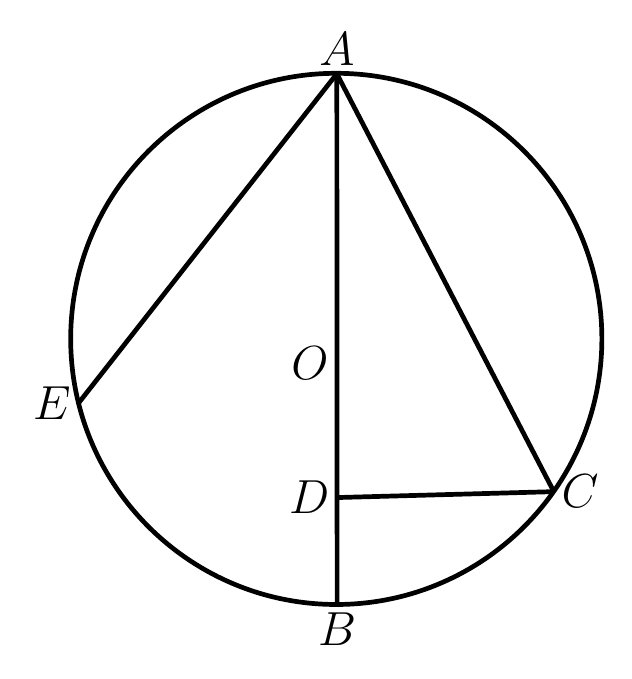
\begin{tikzpicture}[line join=round, line width=1.7pt,
  lbl/.style={font=\fontsize{18}{21.6}\selectfont, inner sep=2pt}]
  % Named coordinates (scale s = 0.021448 cm/px, origin at circle centre O)
  \coordinate (O) at (0,0);
  \coordinate (A) at (0.007,3.367);
  \coordinate (B) at (0.011,-3.373);
  \coordinate (C) at (2.763,-1.940);
  \coordinate (D) at (0.011,-2.015);
  \coordinate (E) at (-3.273,-0.815);

  % Circle, radius 157.27 px
  \draw (O) circle[radius=3.373];

  % Diameter AB
  \draw (A) -- (B);

  % Chords AC and AE
  \draw (A) -- (C);
  \draw (A) -- (E);

  % Segment DC
  \draw (D) -- (C);

  % Labels
  \node[lbl, above] at (A) {$A$};
  \node[lbl, below] at (B) {$B$};
  \node[lbl, right] at (C) {$C$};
  \node[lbl, left] at (D) {$D$};
  \node[lbl, left] at (E) {$E$};
  \node[lbl, below left] at (O) {$O$};
\end{tikzpicture}
\end{document}